\chapter{Results} \label{sec:results}
To benchmark the hybrid technique we employ the method on a number of model problems. In all of the following simulations we use a weight of uniform weight of $0.5$ for both the discrete and continuum components in the hybrid zones. Unless otherwise stated, the simulations utilized an MPM cell width to DEM grain diameter ratio of 2:1. We also utilize the hyperelastic formulation to model the continuum regions in all simulations. 

\begin{table}[!htb]
  %\begin{tabular}{|p{1.7cm}|p{0.7cm}|p{1.0cm}|p{0.7cm}|p{0.8cm}|p{1.0cm}|}
  \begin{tabular}{llllll}
      \hline
      \textbf{Simulation} & \textbf{DEM Cost} & \textbf{Hybrid Cost} & \textbf{Total Cost} & \textbf{Speedup} & \textbf{DEM Grains}\\
      \hline
      Silo, DEM    & 0.41 & N/A & 0.41 & N/A  & 100,000\\
      Silo, Hybrid & 0.25 & 0.03 & 0.28 & $1.47\times$ & 78,538\\
      \hline
      Toss, DEM    & 0.620 & N/A & 0.620 & N/A  & 120,000\\
      Toss, Hybrid & 0.164 & 0.193 & 0.357 & $1.74\times$ & 28,289\\
      \hline
      Drill, DEM    & 1.84  & N/A  & 1.84  & N/A & 360,000\\
      Drill, Hybrid & 0.125 & 0.145 & 0.27 & $6.82\times$ & 42,933\\
      \hline
      Tires, DEM    & 3.60 & N/A & 3.60 & N/A  & 588,320\\
      Tires, Hybrid & 0.54 & 0.51 & 1.05 & $3.43\times$ & 114,35\\
      \hline
  \end{tabular}
  \vspace{0.2cm}
  \caption{Simulation performance. Timings of our hybrid approach compared to a purely discrete approach for different scenarios. All reported costs have units of average seconds per time step. The hybrid cost includes both the cost of MPM time evolution and the coupling solves. We take a constant DEM time step of $dt=10^{-6}$ and a constant MPM time step of $dt=10^{-5}$. We gathered all performance statistics on an Intel 3.5 GHz Core i7-4770K with a single thread.} \label{tbl:speedup}
\end{table}

%\input{result_granular_column_collapse.tex}

%\input{result_silo_discharge.tex}

%\input{result_bunny_drill.tex}

%\input{result_drum.tex}

%\input{result_speedup.tex}

%\input{result_core_scaling.tex}

\section{Granular Column Collapse}
In Fig.~\ref{fig:hybrid:column_collapse}, we simulate a collapsing column
with pure DEM and with our hybrid approach. Note the correspondence between the shapes of both
piles. Further observe that our hybrid method captures detailed ``fly away'' effects -- individual grains
separate from the overall bulk and roll away at the front of the collapse, a visually important effect that
would be difficult to capture with a purely continuum model.

\begin{figure}
  \centering
  \includegraphics[width=0.8\linewidth]{figs/column_collapse.pdf}
  %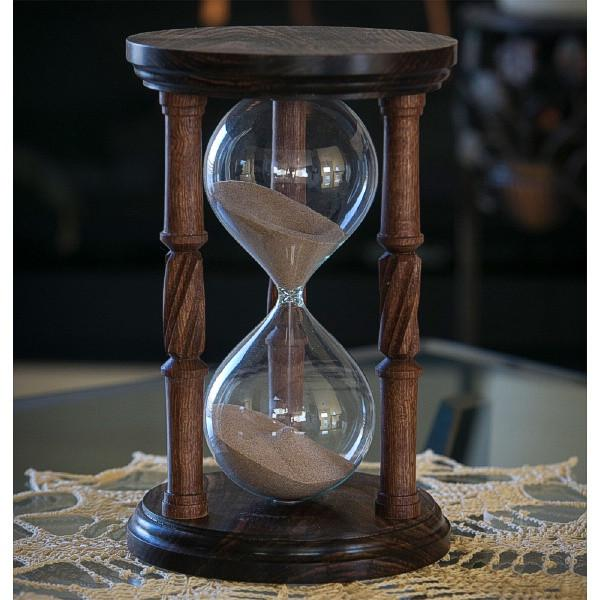
\includegraphics[width=0.4\textwidth]{figs/hourglass_whole.jpg}
  \caption{
    Granular column: A collapsing column simulated with DEM (top) and with our hybrid approach
    (bottom). Observe the nice agreement in the final profile with our hybrid approach and the purely DEM approach.
  }
  \label{fig:hybrid:column_collapse}
\end{figure}

Encouraged by the agreement between the pure DEM approach and our hybrid approach, we validated our hybrid
model against the power-law scaling of the run-out distance $\delta d = d_f - d_i$ reported in the literature,  
where $d_f$ is the distance from the left wall (for a unilateral collapse like our study, or from the column center for a bilateral collapse) to the center of mass of the foremost grain that is connected to the main collection of grains, and $d_i$ is the initial column width (for a unilateral collapse, or the initial half-width for a bilateral one), as in Fig.~\ref{fig:hybrid:column_collapse}.
Granular run-out in a column follows a power law scaling as a function of the initial aspect ratio $AR = h_i / d_i$ in both experimental \cite{Lube:2005,Balmforth:2005}
and numerical \cite{Staron:2005,Lagree:2011,Mast:2015,Dunatunga:2015:Continuum} tests, where $h_i$ is the initial height of the column. Running a series of run-out
simulations over a range of aspect ratios, we corroborate the previously reported power law scaling.
Below a critical aspect ratio, we observe a linear run-out distance as a function of aspect ratio. Above this
threshold, we observe a second power law scaling.

\begin{figure}
  \centering
  \includegraphics[width=0.7\linewidth]{figs/runout_curve.pdf}
  %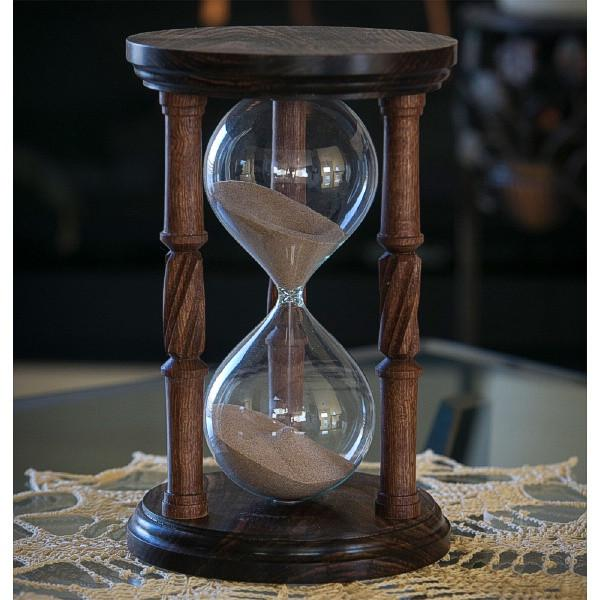
\includegraphics[width=0.4\textwidth]{figs/hourglass_whole.jpg}
  \caption{
    Runout of a 2D granular column: Nondimensionalized runout distance, $\delta d/d_i=(d_f-d_i) / d_i$, vs aspect ratio, $AR = h_i / d_i$. Like DEM, our hybrid technique captures the two distinct regimes that Lube \cite{Lube:2005} observed in experiments. We perform a linear fit in the low-$AR$ regime, and a power-law fit in the high-$AR$ regime.}
  \label{fig:hybrid:runout_curve}
\end{figure}

As evident in Fig.~\ref{fig:hybrid:runout_curve}, a pure discrete simulation captures the expected runout profile. Encouragingly, our hybrid method
captures a similar runout profile, with a clear turnover point. In the aforementioned experimental study by Lube, experiments showed that for AR $<$ 1.8, the runout profile could be described
by a simple linear relation:  $\delta d/d_i=\alpha(AR)$. Lube found $\alpha = 1.2$ while our simulation data fits best with with $\alpha = 1.45$. 
In regimes with AR $>$ 2.8, the runout distance was best described with a power law of the form  $\delta d/d_i=\beta(AR)^\gamma$. Lube observed a best-fit with $\beta = 1.9$ and $\gamma = 0.67$. In comparison, our data fits best with $\beta = 2.05$ and $\gamma = 0.67$. We thus obtain a good quantitative match to experimental results.

\begin{figure}
  \centering
  \includegraphics[width=0.8\linewidth]{figs/column_collapse_3d_brighter.pdf}
  %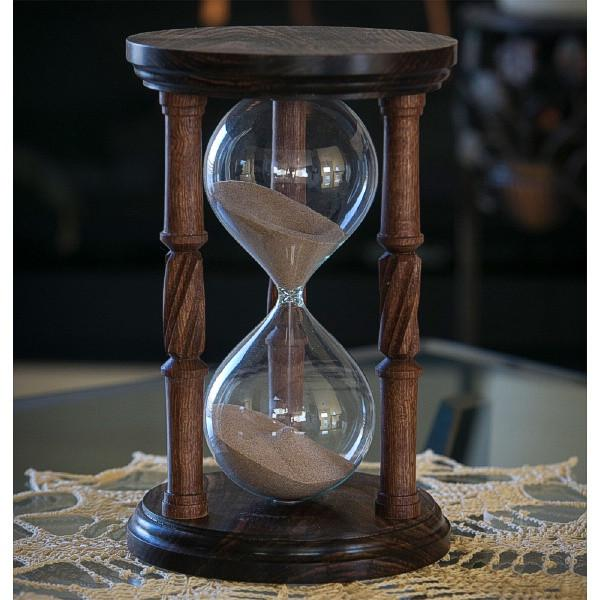
\includegraphics[width=0.4\textwidth]{figs/hourglass_whole.jpg}
  \caption{
    3D column collapse: a column collapse simulated with DEM (left) and with our hybrid method (right) at the same snapshots in time.
  }
  \label{fig:hybrid:column_collapse_3d}
\end{figure}

Extending to 3D, we also obtain a good qualitative matchup of the collapse in motion. Fig.~\ref{fig:hybrid:column_collapse_3d} shows the motion of a discrete and a hybrid column collapse.
Again note the grains at the edge of the runout, which the hybrid technique is able to capture.

\section{Silo Discharge}
In Fig.~\ref{fig:hybrid:silo_discharge}, we simulate a silo that discharges grains using a purely discrete approach and our hybrid approach.
With our approach, the oracle identifies the interior of the
initial mass of grains as a continuum. As grains exit the silo and the continuum region falls towards the orifice, our
method automatically converts the continuum material to discrete material. As grains form a pile on the ground, our
method detects the formation of the sufficiently dense portions of the pile and automatically converts discrete grains
to continuum material points in this area.

\begin{center}
  \centering
  \includegraphics[width=0.8\linewidth]{figs/silo_larger.pdf}
  %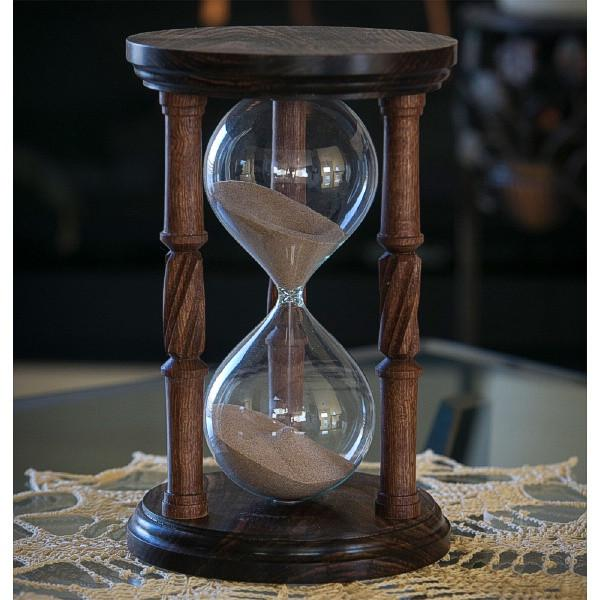
\includegraphics[width=0.4\textwidth]{figs/hourglass_whole.jpg}
  \captionof{figure}{
    Silo discharge: A silo discharges grains with a discrete method (left) and with our hybrid method (right).
  }
  \label{fig:hybrid:silo_discharge}
\end{center}

The hybrid 2D hourglass has a slightly faster flow rate than the discrete only counterpart. We believe that the ability to control the coordination number for newly sampled DEM particles would reconcile these flow rates. Generating packings given constraints is an interesting avenue of future work.

\begin{center}
  \centering
  \includegraphics[width=0.5\linewidth]{figs/bouncing_silo/hybrid/combine.pdf}
  %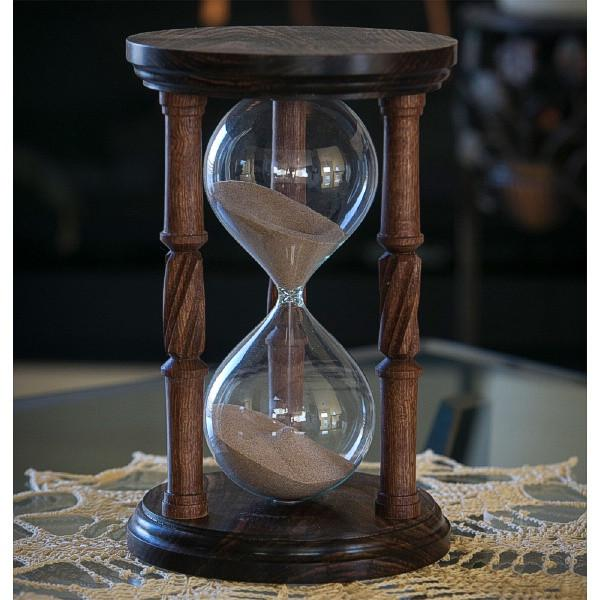
\includegraphics[width=0.4\textwidth]{figs/hourglass_whole.jpg}
  \captionof{figure}{
    3D silo discharge simulated with our hybrid approach: Left is a full view of the discharging grains while right is a cutaway view.
  }
  \label{fig:hybrid:silo_discharge_3d}
\end{center}

We also simulate a hybrid silo discharge in 3D (Fig.~\ref{fig:hybrid:silo_discharge_3d}). The hybrid approach is able to model ballistic motion and collisions after grains flowing from the silo enter a "gaseous" state. This ability to model contact is crucial for capturing the asymmetrical shape of the column, as well as the ballistic bounces when grains impact the container and the pile, both of which are observed in real-life hourglasses.
\begin{center}
  \centering
  \includegraphics[width=0.5\linewidth]{figs/bouncing_silo.pdf}
  %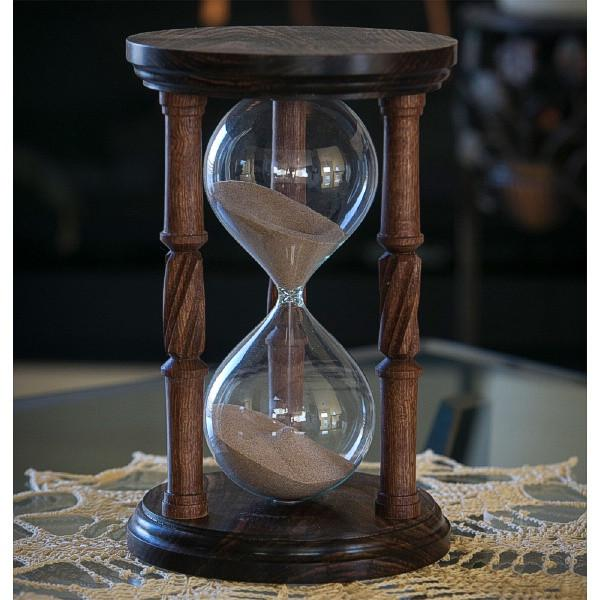
\includegraphics[width=0.4\textwidth]{figs/hourglass_whole.jpg}
  \captionof{figure}{Silo discharge (3D large orifice, $r=1.8$): Top: with $0$ restitution, the flow looks uniform. Middle: with $e=0.5$, the flow appears more energetic, with multiple fly away grains. The pure MPM version of this simulation (bottom) has a less energetic flow and fails to simulate grains bouncing away from the bulk.}
  \label{COR-compare}
\end{center}

MPM fails at simulating fly away grains, as the Particle-in-Cell method handles collisions by homogenizing each Lagrangian particle's velocity onto a background Eulerian grid and then transferring back. This series of operations results in an effectively inelastic collision among Lagrangian particles, i.e. with restitution coefficient $e = 0$. Note that this inelastic nature is independent of the particle-grid transfer scheme, i.e. PIC, FLIP, or APIC.

In contrast, our hybrid approach handles the full range of restitution coefficients from $0$ to $1$, due to the fact that we handle these collisions via DEM. In Fig.~\ref{COR-compare}, we show a comparison between $e=0$ and $e=0.5$. Note that the MPM counterpart is simulated with sticky boundary conditions on the bottom. Notice that when $e=0$, the hybrid approach results in the expected behavior of less energetic-appearing grains. It fails to capture the detailed bouncing effects and has a more uniform shape and flow profile.
\begin{center}
  \centering
  \includegraphics[width=0.8\linewidth]{figs/jamming.pdf}
  %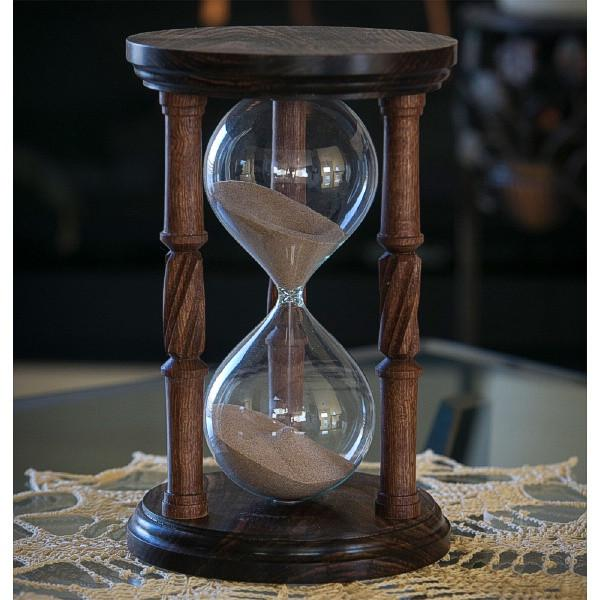
\includegraphics[width=0.4\textwidth]{figs/hourglass_whole.jpg}
  \captionof{figure}{
    Silo discharge (small orifice, $r=0.2$): A silo discharges grains with a discrete method (left), our hybrid
    method (middle), and a continuum method (right). Both the discrete and hybrid approach capture size-dependent clogging effects, and
    all flow from the orifice halts. The continuum simulation, in contrast, flows nonphysically.
  }
  \label{fig:hybrid:silo_frictoinal_jam}
\end{center}
Another advantage of our hybrid approach over a purely continuum method is the ability to frictionally
jam due to so-called finite size effects. In Fig.~\ref{fig:hybrid:silo_frictoinal_jam}, we simulate a silo discharge with a small orifice
width using a purely DEM algorithm, our hybrid algorithm, and a purely continuum algorithm. Note that we use an MPM cell width to DEM mean grain diameter ratio of 1:1 to more accurately couple the hybrid region near the orifice. Our hybrid simulation, like the purely DEM simulation, jams with the small orifice width, as expected. On the contrary the continuum, regardless of the grid resolution, fails to capture these finite size effects. Extra non-local modeling is needed \cite{Kamrin:2014}.

\section{Penetrometer Insertion}
\begin{figure}
  \centering
  \includegraphics[width=0.8\linewidth]{figs/stake_insertion.pdf}
  %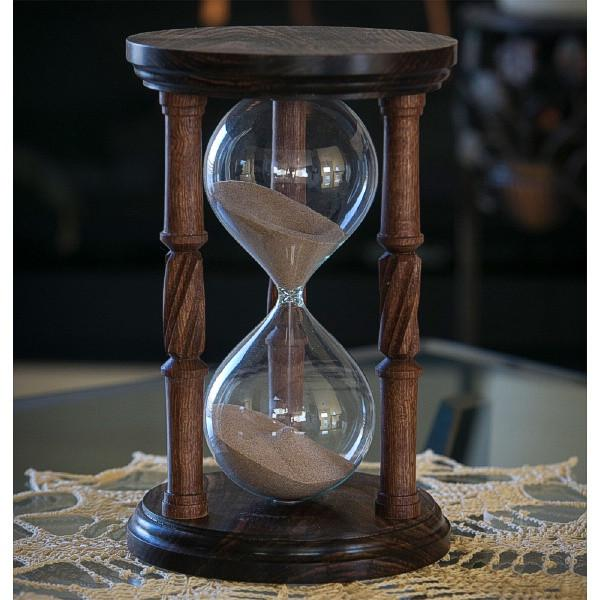
\includegraphics[width=0.4\textwidth]{figs/hourglass_whole.jpg}
  \caption{
    Penetrometer insertion: We insert a penetrometer into a bed of grains with our hybrid algorithm (first four frames).
    As the penetrometer enters the bed, our hybrid oracle identifies the region around the tip as requiring a discrete
    treatment and enriches the simulation domain in this area. As the simulation progresses, the continuum region
    eventually experiences a topology change and splits in two. Examining an overlay of a hybrid simulation (purple) on a purely discrete simulation (peach), we find the resulting profiles to be in almost perfect agreement (rightmost frame).
  }
  \label{fig:hybrid:stake_insertion}
\end{figure}

% \todo{{\bf Interaction with general rigid bodies}:
% Since our method uses discrete element to simulate grains on the free surfaces, it naturally handles interactions with general rigid bodies.}

Similar to Yan et al.~\cite{Yan:2010} and Wellmann and Wriggers \cite{Wellmann:2012}, we perform a hybrid
simulation of a penetrometer insertion into a bed of grains (Fig. \ref{fig:hybrid:stake_insertion}). These simulations
are difficult to perform directly with standard continuum methods owing to the massive plastic shape changes observed
around the penetrometer tip. Unlike previous works, we do not specify the region to be treated with DEM
a-priori. Instead, as the penetrometer advances into the bed of grains, our hybrid method is able to
enrich the region surrounding the penetrometer, ensuring that it always interacts with the bed through discrete grains.
As the penetrometer is fully inserted into the bed, the original single continuum region is split in two. Our hybrid
approach gracefully treats this topological change with no extra machinery.

\section{Bunny Toss}
\begin{center}
  \centering
  \includegraphics[width=0.4\linewidth]{figs/bunny_drill/toss_config_0032_COR00.pdf}
  \captionof{figure}{The bunny crashes into a container of gumballs with different coefficients of restitution using our hybrid method.}
  \label{fig:hybrid:bunny_toss}
\end{center}
We initialize a bunny with non-zero translational and angular velocity and simulate the resulting collision 
with a packing of gumballs. This high-speed bunny produces a splash upon impact with the gumballs before coming to rest.
In Fig.~\ref{fig:hybrid:bunny_toss}, the top simulation has zero restitution, while the bottom simulation has restitution of $e = 0.5$.
The larger coefficient of restitution leads to a simulation with a more dynamic splash.

While DEM uses 120,000 grains to simulate this scene, our hybrid approach only uses an average of 28,289 grains. In total, taking into account of the cost of MPM and the coupling computation (where again the MPM cell width is $2\times$ the mean grain diameter), our method is $1.74\times$ faster than DEM (Table \ref{tbl:speedup}).

\section{Excavator}
\begin{center}
\centering
  \includegraphics[width=0.4\linewidth]{figs/bunny_drill/excavator.pdf}
  %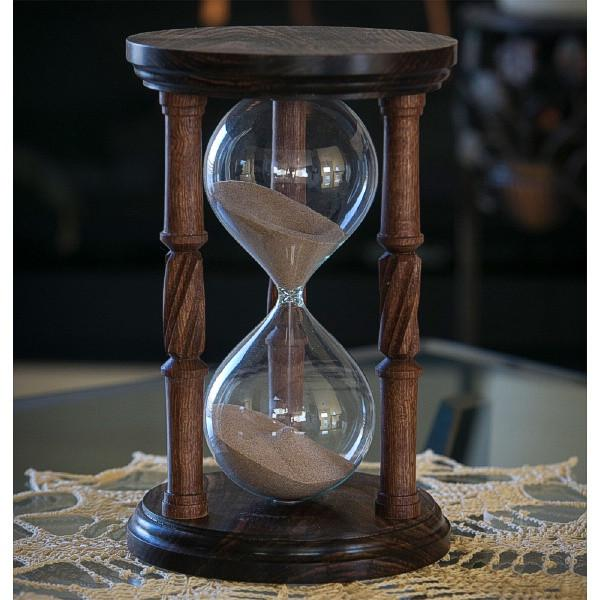
\includegraphics[width=0.4\textwidth]{figs/hourglass_whole.jpg}
  \captionof{figure}{We script an excavator to scoop gumballs out of a container.}
  \label{fig:hybrid:excavator}
\end{center}

In Fig.~\ref{fig:hybrid:excavator}, we script an excavator to scoop gumballs from the same container as the bunny toss. Our hybrid oracle robustly handles topology changes in the simulation domain induced by the excavator. Although not visible, as the excavator enters the granular pile, the continuum elements directly below the top DEM and hybrid layers are enriched to DEM grains. As the excavator digs in and rotates through the pile, it only interacts with DEM grains. material, it only  As we employ the same granular packing as the bunny toss in this test, we obtain a comparable speedup to that example.

\section{Bunny Drill}
 \begin{center}
 \centering
 \includegraphics[width=1.0\textwidth]{figs/bunny_drill.pdf}
 \captionof{figure}{Four rigid bunnies are scripted to rapidly rotate about the vertical axis while simultaneously moving into and out of a packing of 360,000 grains. The bunnies inject a large amount of energy into the system, causing significant displacement of grains in the interior while also producing an energetic splash near the free surface. From left to right we show: a cutaway view of initial conditions for a hybrid simulation, a cutaway frame from when the bunnies have penetrated the surface, a top down view of the same frame, and a cutaway view of purely discrete simulation at the same frame.}
 \label{fig:hybrid:bunny_drill}
 \end{center}
 
We aggressively insert and remove four scripted bunnies from a pile of 360,000 grains (Fig.~\ref{fig:hybrid:bunny_drill}). While initially only the top surface is represented as discrete grains, our method is able to dynamically enrich the interior around the bunnies in response to their motion. Our hybrid method obtains a similar visual result compared to the pure DEM simulation, yet it uses $88\%$ fewer discrete grains and is thus $6.82\times$ faster (See Table ~\ref{tbl:speedup}).

The bunny drill provides a key example of when the hybrid method is useful. While visually the only grains seen from the observer are the grains at the top of the container, the behavior of those flyaway grains are directly impacted by the physics of the granular layer underneath. By still solving for physics while the bunnies are not visible we enhance the final result, while still retaining a speedup over a pure discrete simulation that would capture similar visible granular dynamics. Also much like the excavator example, as the bunnies move through the interior of the domain, they are constantly kept in contact with discrete grains, so that any momentum transfers occur at bunny-DEM interfaces. This does away with the need to introduce continuum contact laws. Another advantage of the hybrid technique is thus shown: while we use the DEM to simplify the need to derive complicated constitutive laws in the continuum, we also use the DEM to simplify contact laws with rigid bodies.

\section{Tires on Gravel Road}
\begin{center}
  \centering
  \includegraphics[width=0.4\textwidth]{figs/bunny_drill/tire/config_0000_single_cropped.png}
  \includegraphics[width=0.4\textwidth]{figs/bunny_drill/tire/config_0066_speed_multi.png}
  \includegraphics[width=0.4\textwidth]{figs/bunny_drill/tire/config_0052_density.png}
  %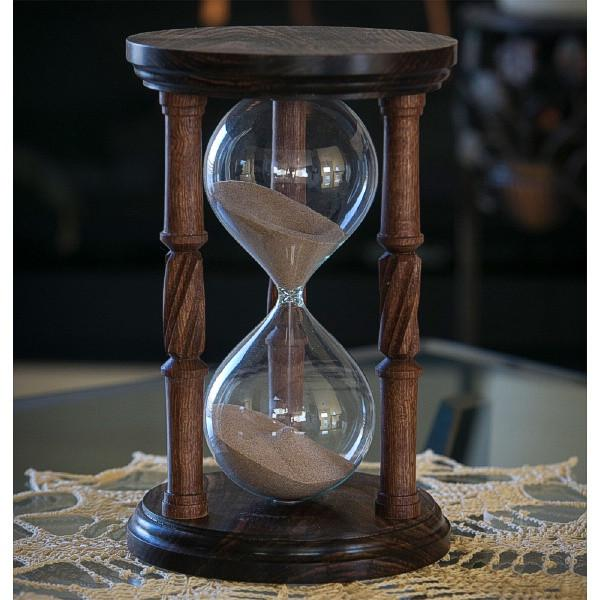
\includegraphics[width=0.4\textwidth]{figs/hourglass_whole.jpg}
  %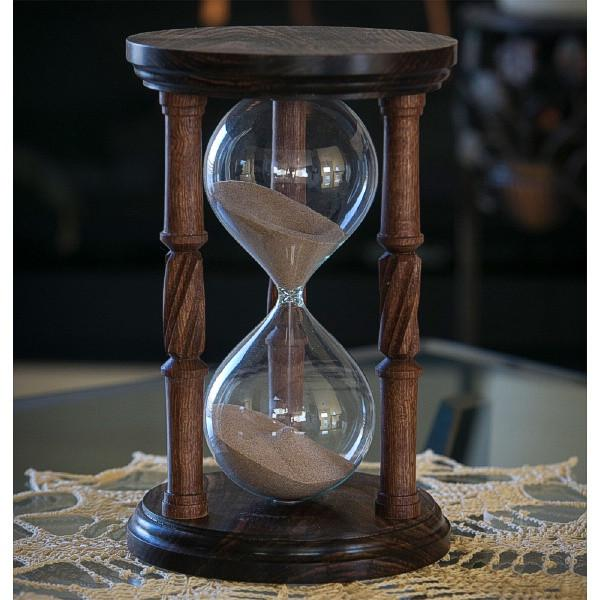
\includegraphics[width=0.4\textwidth]{figs/hourglass_whole.jpg}
  %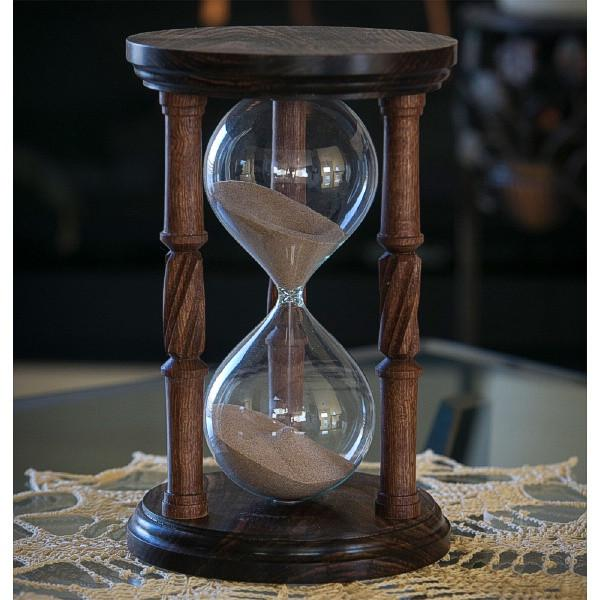
\includegraphics[width=0.4\textwidth]{figs/hourglass_whole.jpg}
  \captionof{figure}{Simulations of tires traversing a bed of gravel. Left: A render of the initial condition (boundary condition not shown), with a tire poised to race across the bed of grains. Notice the layered hybridization employed here. Center: Tires with different angular velocities but equal densities. Left to right the tires rotate at 1000 rad/s, 100 rad/s, and 10 rad/s. The 1000 rad/s tire produces a large granular splash while the 10 rad/s tire produces almost no splash. Right: Tires of different densities, but with the same angular velocities. Left to right the tires have $5\times$, $2\times$, and $1\times$ the density of gravel. As the tires traverse the system, the larger density tires sink into the gravel.}
  \label{fig:hybrid:tire}
\end{center}
On a slightly less whimsical note and to test our method on a more real world example, we simulate off-road tires traversing a gravel road. The tires are given a constant angular velocity around each of their axes, but are otherwise dynamically simulated. The hybrid method is able to capture multiple effects such as large splashes when fast rotating wheels collide with the grains, as well as tires sinking into the pile of grains due to a large density difference. While simulating this scene with a pure discrete method requires 822,956 grains, our hybrid approach allows us to simulate only a thin layer of discrete grains and the remainder is continuum (Fig.~\ref{fig:hybrid:tire} (a)). Here, the MPM cell width is $1.75\times$ the mean grain diameter. On average, the hybrid approach is $3.43\times$ faster than a purely discrete method (Table ~\ref{tbl:speedup}).

Again, as the tires dig through the domain, DEM grains are constantly being enriched, so that the entires only interact with those grains. The enrichment also provides a source for grains that are splayed back behind the tire.

\section{Spinning Drum}

\begin{center}
  \centering
  \includegraphics[width=0.8\linewidth]{figs/drum.pdf}
  %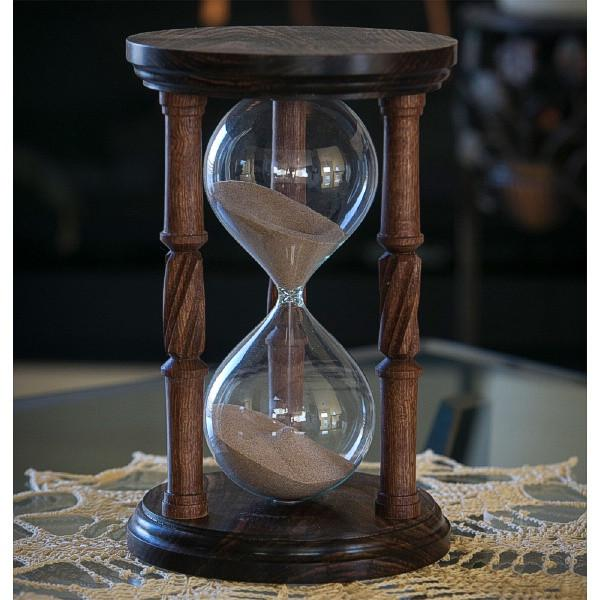
\includegraphics[width=0.4\textwidth]{figs/hourglass_whole.jpg}
  \captionof{figure}{
    Spinning drum: We rotate a drum filled halfway with grains using DEM (top row) and using our
    hybrid algorithm (bottom row). As the system evolves, observe that the shape of the free surface obtained with our
    hybrid method agrees with that of the purely discrete method.
  }
  \label{fig:hybrid:spinning_drum}
\end{center}

Continuing the theme of more practical applications, we simulate the flow of grains in a spinning drum. An understanding of drum geometries is important in industrial applications (e.g. mills,
tumblers) and in the study of free-surface flows \cite{Midi:2004:Dense}. To assess whether our algorithm is
suitable for these geometries, we fill a drum with grains to half its area, and impose a rotation to the drum with
a constant angular velocity.

With a pure DEM simulation, we observe nearly rigid grains near the base of the drum, a steadily increasing flow towards the interior of the granular assembly, and loosely packed grains near the free surface. As the transient phase subsides, we observe the characteristic free-surface shape. Our pure DEM simulation thus matches physical experiment and other numerical simulation, providing a baseline of comparison.

Thus comparing the purely discrete results to those from our hybrid algorithm (Fig.~\ref{fig:hybrid:spinning_drum}), we find
the profiles to be in good agreement throughout the simulation. Because our hybrid algorithm treats
regions near surfaces with discrete grains, we do not require any additional machinery to handle the drum boundary
condition beyond that from the discrete simulation. Again, we demonstrate the advantage of the hybrid algorithm in treating interactions with boundaries and rigid objects. Like the discrete simulation, our hybrid algorithm is also able to
capture free flight fly away grains near the top of the domain.

\section{Speedup Study}
\begin{center}
  \centering
  \includegraphics[width=0.6\linewidth]{figs/chute_flow.pdf}
  %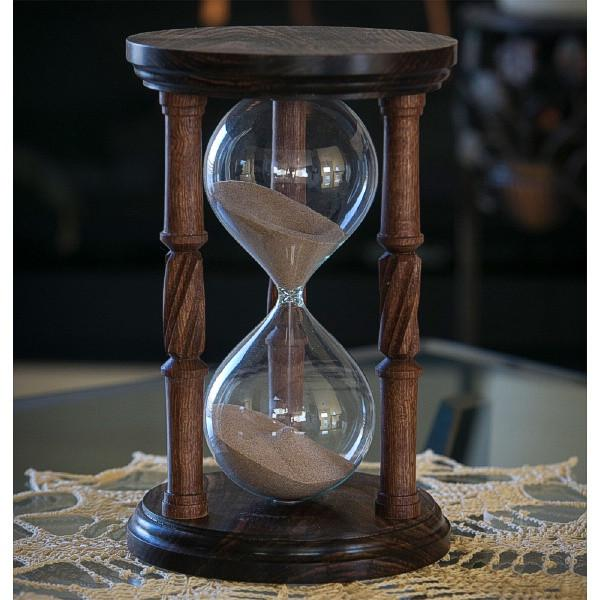
\includegraphics[width=0.4\textwidth]{figs/hourglass_whole.jpg}
  \captionof{figure}{
    Periodic chute flow: We set a granular packing at an angle $\theta$ with periodic boundary conditions to simulate flow down a chute.
  }
  \label{fig:hybrid:chute_flow}
\end{center}

We seek to quantify the speedup we are able to obtain from the hybrid
method over a pure discrete simulation. In order to do this, we use the geometry, seen in
Fig.~\ref{fig:hybrid:chute_flow}. Grains are initialized in a column and are then tilted at an angle $\theta$ relative
to the horizontal, with gravity applied. We then apply periodic boundary conditions, causing a continual 
flow of grains down-slope. Three factors are adjusted: the initial total number of grains $N_i$ before hybridization, the fraction of DEM left
after the hybridization $F$, and the hybrid grid size (identical to the MPM grid size here) $H$. A parametric sweep
over these variables allows for the construction of a phase plot, which shows for a given $N_i$, when a 
pure discrete simulation with $N_i$ grains is faster or slower than a hybrid simulation initialized with $N_i$ grains but with
different $F$ and $H$. Note that the geometry is kept fixed for all simulations, so that increasing or decreasing $N_i$ means
decreasing or increasing the average grain diameter.

\begin{figure}
  \centering
  \includegraphics[width=0.75\linewidth]{figs/phase_plots2.pdf}
  %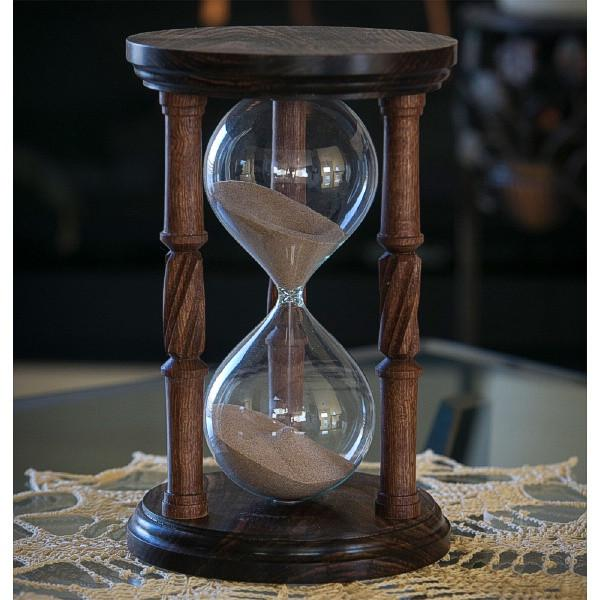
\includegraphics[width=0.4\textwidth]{figs/hourglass_whole.jpg}
  \caption{
    Phase plots: Phase plots for $H = 0.0025$ (top left), $H = 0.00125$ (top right), $H = 0.00083$ (bottom left), and $H = 0.000625$ (bottom right). Red denotes
    regimes where our hybrid scheme is faster while blue denotes regimes where DEM is faster.
  }
  \label{fig:hybrid:phase_plots}
\end{figure}

$N_i$ ranges from 1,000 grains up to 156,000 grains, $F$ ranges from $0.07$ to $0.89$, and $H$ ranges from $0.0025$ to $0.000625$. Cell width to mean grain diameter ratios thus range from 19:1 to 0.4:1.
Fig.~\ref{fig:hybrid:phase_plots} displays phase plots over different values of $H$. As $H$ decreases, more elements are hybridized, and so computational costs associated
with hybridization increase. However, even for the most refined grid, a speedup can still be obtained with a reasonable $F$ for a simulation requiring 40,000 grains or more.
It can be seen from Fig.~\ref{fig:hybrid:phase_plots} that a speedup on the order of $12\times$ can be obtained. While it may seem that increasing the resolution (thus decreasing $H$)
results in a decay of the maximum speedup obtained, one can exploit a characteristic of a smaller $H$: with smaller $H$, a smaller $F$ can be obtained.

Looking at the relationship between $H$ and $F$ from a different perspective, an analysis of the speedup for layered hybridization in 2D can be conducted from the geometry of the problem. Letting $C_D$ be the computational cost
of a discrete grain, $C_E$ the cost of enrichment for a hybrid cell, $C_C$ the cost for a continuum element, and $A$ the effective total number of grains (average number of grains per 
cell multiplied with the number of cells containing grains), we obtain the following expression for the total time $T_H$ for a complete hybrid iteration and total time $T_C$ for a pure discrete simulation:

\begin{align}
\begin{aligned}
T_H &= C_EhN^2 +C_D\frac{(N_D+N_H)N}{hN^2}+C_C(hN-N_D)N , \\
T_C &= C_DA.
\end{aligned}
\end{align}

A reduction ratio $R_A$ can then be defined between the computational time of a hybrid simulation and an equivalent discrete simulation of $A$ grains:

\begin{align}
R_A &=\frac{T_H}{T_C}=\frac{C_E h N^2}{C_DA} +\frac{C_D (N_D+N_H)N}{hN}+\frac{C_C (hN-N_D)N}{C_DA}.
\end{align}

Minimizing $R_A$ results in the largest speedup, 
and we can find the optimal $N$ giving the largest speed up as:
%and it can be shown that $R_A$ can be written as:
\begin{align}
\begin{aligned}
%R_A &=\frac{C_E}{h(C_E+C_C)N}+\frac{2}{hN} +\frac{C_C}{h^2(C_E+C_C)N}\left(h-\frac{1}{N}\right) \\
N & = \left(\frac{C_DA}{h^2(C_E+C_C)}\right)^{1/3}.
\end{aligned}
\end{align}

The key insight is that if $N$ is chosen in the manner shown above in relation to $A$, then as $A\rightarrow\infty$, $R_A\rightarrow0$, which means that increasing speedups
can be had for increasing grain numbers. This is an extremely useful property, and serves to highlight the potential of our hybrid method to tackle problems bridging 
micro/mesoscale causes to macroscale effects. 

For the layered hybridization method in 3D described in Section~\ref{sec:layered_3D}, we obtain the best speedups if $N$ scales with $A$ according to $N \propto A^{1/4}$. Then as $A\rightarrow\infty$, $R_A\rightarrow0$.

It is important to note that $N$ scales with $A$ in the power of $1/4$ ($1/3$ in 2D), not $1/3$ ($1/2$ in 2D).
An intuitive explanation is that if we refine both the discrete and continuum elements equally (this corresponds to setting $N \propto A^{1/3}$ ($N \propto A^{1/2}$ in 2D)) while keeping the discrete layer thickness to a minimum,
then the discrete computation time will scale as $N^2$ ($N$ in 2D) whereas the
continuum will scale as $N^3$ ($N^2$ in 2D), so eventually the continuum computation time will dominate, and we
will hit a bound. However, if we refine them \textit{differently} and maintain a balance between the two (i.e., setting $N \propto A^{1/4}$ in 3D and $N \propto A^{1/3}$ in 2D),
then the acceleration continues.

\section{Core Scaling}
\begin{figure}
  \centering
  \includegraphics[width=0.5\textwidth]{figs/core_scaling.pdf}
  %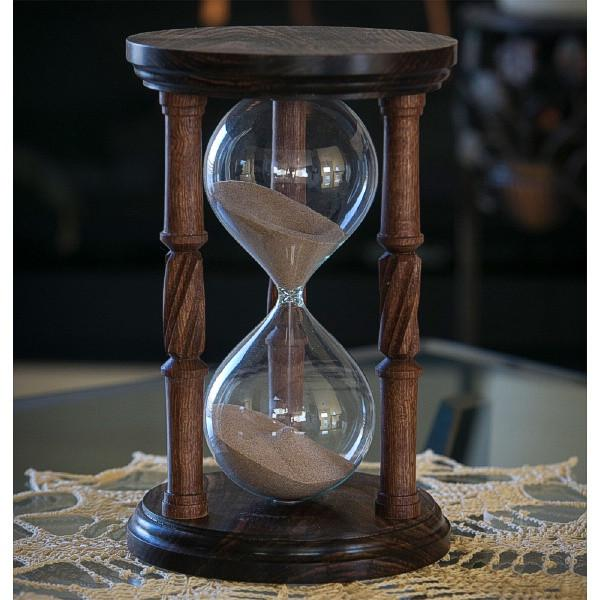
\includegraphics[width=0.4\textwidth]{figs/hourglass_whole.jpg}
  \caption{
    Periodic chute flow: We set a granular packing at an angle $\theta$ with periodic boundary conditions to simulate flow down a chute.
  }
  \label{fig:hybrid:chute_flow}
\end{figure}


It should be noted that while the hybrid technique itself is able to push the domain sizes we are able to simulate, the ability to run in parallel is also crucial for even larger problems. Therefore we require an analysis of how well the code scales with core count.

To study how well our code parallelizes, we conducted a test with the bunny drill example. We ran both a pure DEM and a hybrid simulation of the bunny drill with varying core counts. For each core count, we ran each simulation for two hours of wall clock time and measured the number of completed time steps. 

As evident from Figure \ref{fig:hybrid:chute_flow}, both DEM and our hybrid method do parallelize, albeit with sub-linear scaling. We note that at the time of this test, many routines in the code were not fully parallelized, and a complete refactoring with parallelization in mind would greatly improve scaling. For example, a domain decomposition algorithm across all components of the hybrid solve would result in much closer to linear scaling.



